\documentclass{beamer}
\usepackage[T1]{fontenc}
\usepackage[utf8]{inputenc}
\usepackage{lmodern}
\usepackage[ngerman]{babel}

\usepackage{graphics}

\usepackage{amsmath}
\usepackage{booktabs}
\usepackage{listings}

\usepackage{dot2texi}
\usepackage{tikz}
\usetikzlibrary{arrows,shapes}
 \usetikzlibrary{matrix}
\usetikzlibrary{automata}

\usepackage{wrapfig}

\usetheme{Singapore}
\usecolortheme{dove}
\graphicspath{{images/}{../comics/}}

\newcommand{\xn}{\visible<2->{$\times$}}
\newcommand{\xj}{\visible<2->{$\checkmark$}}
\newcommand{\rd}[1]{\textcolor{red}{#1}}
\newcommand{\gn}[1]{\textcolor{green}{#1}}
\newcommand{\bl}[1]{\textcolor{blue}{#1}}

\newcommand{\hiddencell}[2]{\action<#1->{#2}}

\newcommand{\link}[2][blue]{\underline{\textcolor{#1}{#2}}}
\renewcommand{\emph}[1]{\textit{\textcolor{gray}{#1}}}
\newcommand{\warn}[1]{\textcolor{red}{#1}}
\newcommand{\ans}[2]{\visible<#1->{\textcolor{green!70!black}{#2}}}
\newcommand{\xb}[1]{{\bf #1}}   % \xb {fett}
\newcommand{\xu}{\underline}    % \xu {unterstrichen}
\newcommand{\hide}{\onslide+<+(1)->}

\AtBeginSection[]
{
  \begin{frame}[plain]
    \frametitle{}
    {\footnotesize
      \tableofcontents[currentsection]
    }
  \end{frame}
}

\title{Grundbegriffe der Informatik}
\author{Patrick Niklaus}

\begin{document}
\begin{frame}
  \frametitle{Grundbegriffe der Informatik}
  \framesubtitle{9. Tutorium}
  \begin{description}
    \item \textbf{Name:} Patrick Niklaus
    \item \textbf{E-Mail:} patrick.niklaus@student.kit.edu
    \item \textbf{Nr:} 43
  \end{description}
\end{frame}

\section{Übungsblatt}
\begin{frame}
  \frametitle{Anmerkungen zum letzten Übungsblatt}
  \begin{enumerate}
    \item $f(n) \in \Theta(g(n))$ bedeutet \warn{nicht} $f(n) = c \cdot g(n)$
    \item Die Regel mit "`der höhste Exponent gewinnt"' gilt nur bei Polynomen!
    \item $f(n) \leq c \cdot g(n)$ muss entweder über vollständige Induktion bewiesen werden, oder durch Abschätzen, aber nicht durch "`Einsetzen"'.
  \end{enumerate}
\end{frame}

\section{Endliche Automaten}
\subsection*{}
\begin{frame}
  \frametitle{Arten von Automaten}
  \pause
  \begin{block}{Mealy-Automat}
    \begin{itemize}
      \item Erzeugung einer Ausgabe bei jedem Zustandsübergang
      \item Ausgabefunktion $g: Z \times X \rightarrow Y^*$
      \item Markieren der \emph{Kanten} mit $x_i|y_i$
    \end{itemize}
   \end{block}
  \pause
  \begin{block}{Moore-Automat}
    \begin{itemize}
      \item Erzeugung einer Ausgabe bei Erreichen eines Zustands
      \item Ausgabefunktion $h: Z \rightarrow Y^*$
      \item Markieren der \emph{Zustände} mit $q_i|y_i$ ($q_i$ ist Zustandsname)
    \end{itemize}
  \end{block}

  In beiden Fällen ist die Ausgabe ein Wort $y = y_0\ldots y_{n-1}$ über einem
  Ausgabealphabet $Y$.
\end{frame}

\begin{frame}
  \frametitle{Endlicher Akzeptor}
  Spezialfall eines Moore-Automaten: Ausgabealphabet $Y = \{0, 1\}$
  \begin{definition}
    $A = (Z, z_0, X, f, F)$
    \begin{description}
      \item[$Z$:] Zustandsmenge
      \item[$z_0$:] Startzustand $z_0 \in Z$
      \item[$X$:] Eingabealphabet
      \item[$f$:] $Z \times X \longrightarrow Z$, Zustandsübergangsfunktion
      \item[$F$:] Akzeptierende Zustände
    \end{description}
  \end{definition}
  \begin{itemize}
    \item Ein Wort $w\in X^*$ wird \emph{akzeptiert}, wenn gilt $f^*(z_0,w)\in F$
    \item Die von einem Akzeptor $A$ \emph{akzeptierte formale Sprache} ist $L(A)=\{w \in X^* |f^*(z_0,w)\in F\}$
   \end{itemize}
\end{frame}


\section{Reguläre Ausdrücke}
\subsection{Definitionen}
\begin{frame}
  \frametitle{Definition}
  \emph{Reguläre Ausdrücke} sind eine verbreitete Notation, um reguläre
  Sprachen (Typ-3) zu beschreiben.
	\begin{block}{Syntax}
		\begin{tabular}{c p{0.7\textwidth}}
				\xb{Zeichen} & 	\xb{Bedeutung} \\
				$( )$			& Klammerung von Alternativen\\
				$\cdot$			& Verkettet Ausdrücke\\
				$|$			& trennt Alternativen\\
				$*$			& beliebig häufiges Vorkommen\\
		\end{tabular}
	\end{block}
  \begin{itemize}
      \item $*$ bindet stärker als Verkettung
      \item Verkettung $(R \cdot S)$ bindet stärker als "`oder"' $(R|S)$
  \end{itemize}
\end{frame}

\begin{frame}
  \frametitle{Die Sprache von R}
	\begin{definition}
		Sei $R$ ein regulärer Ausdruck, dann bezeichnet $\langle R \rangle$ die von ihm erzeugte Sprache.
    Es gilt:
    \begin{itemize}
      \item $\langle \emptyset \rangle =\{\}$
      \item Für $a \in A$ ist $\langle a \rangle=\{a\}$
      \item $\langle R_1 | R_2 \rangle = \langle R_1 \rangle \cup \langle R_2 \rangle$
      \item $\langle R_1 R_2 \rangle = \langle R_1 \rangle \cdot \langle R_2 \rangle$
    \end{itemize}
    $R_1$ und $R_2$ sind hier zwei beliebige reguläre Ausdrücke.
	\end{definition}
\end{frame}

\begin{frame}
  \frametitle{Beispiele}
	\begin{exampleblock}{}
    \begin{itemize}
      \item $R_1 = ({(a|b)*}c)|({(c|b)*}a)$
      \item $R_2 = {(a|b|c|\dots|z)*}.jpg$
      \item $R_3 = {(a|b|c|\dots|z)*}@{(a|b|c|\dots|z)*}.{(a|b|c|\dots|z)*}$
      \item $Z := (a|b|c|\dots|z)$\\
            $R_4 = \text{http://}{Z*}.{Z*}(\emptyset|/Z*)*$
    \end{itemize}
	\end{exampleblock}
\end{frame}

\subsection{Aufgaben}
\begin{frame}
  \frametitle{Aufgaben}
  \begin{enumerate}
		\item Welche Wörter erzeugt der reguläre Ausdruck: $R=(a|b)*abb(a|b)*$\\
    \ans{2}{$\langle R \rangle$ enthält alle Wörter mit dem Teilwort $abb$}
		\item Gebe einen regulären Ausdruck für die Sprache aller Wörter die nicht $ab$ enthalten\\
		\ans{2}{$R = {b*} {a*}$}
  \end{enumerate}
\end{frame}

\begin{frame}
  \frametitle{Aufgaben}
  \begin{enumerate}
		\item Welcher reguläre Ausdruck R erzeugt die Sprache $L=\{\epsilon\}$?
      \ans{2}{$\emptyset*$, denn $\langle \emptyset \rangle ^* = \{\}^* = \{\epsilon\}$}
		\item Gebe einen regulären Ausdruck für die Sprache aller Wörter mit mindestens 3 b's an!\\
			\ans{2}{${(a|b)*}{b(a|b)*}{b(a|b)*}{b(a|b)*}$ oder ${a*}{ba*}{ba*}b{(a|b)*}$}
	\end{enumerate}
\end{frame}

\begin{frame}
  \frametitle{Aufgabe}
  Gegeben ist folgende Klasse von Sprachen über dem Alphabet $\Sigma = \{a,b,c\}$:
  \begin{multline*}
    L_n = \{w|
      \text{w enthält genau einmal das Teilwort $w'=a^n$}\\
      \text{das nicht Teil von $a^k$ mit $k > n$ ist.}
          \}
  \end{multline*}
  Gebt einen regulären Ausdruck $R$ für $L_4$ an! (also: $\langle R \rangle = L_4$)\\
  \hfill
  \ans{2}{
    Wir stellen sicher, dass $aaaa$ genau einmal vorkommt, und sonst nur 1, 2, 3 oder mehr $a$'s.
    \begin{multline*}
      R = ( (b|c)* (\emptyset |a|aa|aaa|aaaaaa*)(b|c)(b|c)*)* \\ aaaa (
      (b|c)(b|c)*(\emptyset |a|aa|aaa|aaaaaa* )(b|c)*)*
    \end{multline*}}
\end{frame}

\begin{frame}
  \frametitle{Aufgabe}
	\begin{exampleblock}{}
		Sei $R$ ein regulärer Ausdruck für eine formale Sprache $L=\langle R \rangle$. Konstruiere einen regulärer Ausdruck
  		\begin{enumerate}
        \item für $L^*$ \\
          \ans{2}{$R_* = (R)*$}
        \item für $L^+$ \\
          \ans{2}{$R_+ = R(R)*$}
  		\end{enumerate}
	\end{exampleblock}
\end{frame}


\section{Rechtslineare Grammatiken}
\subsection{Definition}
\begin{frame}
	\frametitle{rechtslineare Grammatiken}
	\begin{definition}
  		Eine rechtslineare Grammatik ist eine kontextfreie Grammatik $G=(N,T,S,P)$ mit folgenden Einschränkungen:\\
      Alle Produktion sind von der Form:
  		\begin{description}
        \item[] $X \rightarrow w$
        \item[] $X \rightarrow wY$ \hfill ($w \in T^*$\hspace{0.25em} $X,Y \in N$)
  		\end{description}
	\end{definition}
\end{frame}
\begin{frame}
  \frametitle{Äquivalenz}
   Zu jeder rechtslinearen Grammatik gibt es:
	\begin{itemize}
		\item \ldots einen entsprechenden regulären Ausdruck und \pause
		\item \ldots einen einen deterministischen endlichen Automaten
   \end{itemize}
\end{frame}

\subsection{Beispiele}
\begin{frame}
	\frametitle{Rechtslinear?}
	\begin{exampleblock}{Ist diese Grammatik rechtslinear?}
    $G=(\{X,Y\},\{a,b\},X,\{X \rightarrow aY | \epsilon, Y \rightarrow Xb\})$\\
    \begin{description}
      \visible<2->{\item[\emph{nicht} rechtslinear:] Betrachte die Produktion $Y \rightarrow Xb$
      \visible<3->{\item[erzeugte Sprache:] $L(G)=\{a^k b^k | k \in \mathbb N_0 \}$}\\}
    \end{description}
	\end{exampleblock}
  \visible<4->{Kann es eine rechtslineare Grammatik für diese Sprache geben? \\ Ist diese Sprache regulär?}
  \visible<5->{\warn{Nein, ist sie nicht!}}
\end{frame}

\subsection{Aufgaben}
\begin{frame}
\frametitle{Aufgabe}
	\begin{block}{Grammatik $\rightarrow$ Automat}
		$G=(\{X,Y,Z\},\{a,b\},X,P)$\\
    $P=\{X \rightarrow aX | bY | \epsilon, Y \rightarrow aX | bZ | \epsilon, Z \rightarrow aZ | bZ \}$
    \begin{enumerate}
			\item Was ist $L(G)$?
			\item Geben Sie einen endlichen Automaten an, der L(G) akzeptiert.
			\item Lässt sich diese Grammatik noch vereinfachen?
    \end{enumerate}
	\end{block}
	\visible<2->{
	\begin{block}{Lösung}
      		\begin{tikzpicture}[shorten >=1pt,node distance=2cm,auto,initial text=,>=stealth]
        		\node[state,initial,accepting]  (q_0)                       {$0$};
       			\node[state,accepting]          (q_1) [right of= q_0] {$1$};
        		\node[state]                    (q_2) [right of= q_1] {$2$};
        		\path[->] (q_0) edge [loop below]      node        {$a$} ()
        		edge [bend right] node [swap] {$b$} (q_1)
        		(q_1) edge              node        {$b$} (q_2)
        		edge [bend right] node [swap] {$a$} (q_0)
        		(q_2) edge [loop below] node        {$a,b$} ()
        		;
      		\end{tikzpicture}
	\end{block}
	}
\end{frame}


% Nur falls noch Bedarf besteht.
% \section{Strukturelle Induktion}

\subsection*{}
\begin{frame}
  \frametitle{Motivation}
  Wir wollen die vollständige Induktion "verallgemeinern".
  Vorgehen:
  \begin{enumerate}
    \item Aussage für "grundlegende Elemente" beweisen.
    \item Beweisen das die Aussage auch für daraus zusammen gesetzte Elemente gilt.
  \end{enumerate}
\end{frame}
\begin{frame}
  \frametitle{Beispiel}
  Die Menge $M \subseteq \mathbb{Z}^2$ sei wie folgt definiert:
  \begin{itemize}
    \item $(3, 2) \in M$
    \item Wenn $(m, n) \in M$, dann ist auch $(3m - 2n, m) \in M$
    \item Keine weiteren Elemente liegen in $M$.
  \end{itemize}
  \begin{exampleblock}{Aufgabe}
    Zeigen Sie: $\forall m \in M: \exists k \in \mathbb{N}_0: m = (2^{k+1}+1, 2^k + 1)$
  \end{exampleblock}
\end{frame}


\section{Abschluss}
\subsection{Zusammenfassung}
\begin{frame}
  \frametitle{Was ihr jetzt wissen sollte.}
  \begin{enumerate}
    \item Was sind Akzeptoren?
    \item Was sind reguläre Ausdrücke?
    \item Wie kann ich eine Sprache zu einem regulären Ausdruck erzeugen?
    \item Zu was sind rechtslineare Grammatiken äquivalent?
    \item Kann jede reguläre Sprache von einem endlichen Akzeptor erkannt werden?
  \end{enumerate}
\end{frame}

\subsection{xkcd}
\begin{frame}[plain]
  \begin{figure}
    \begin{center}
      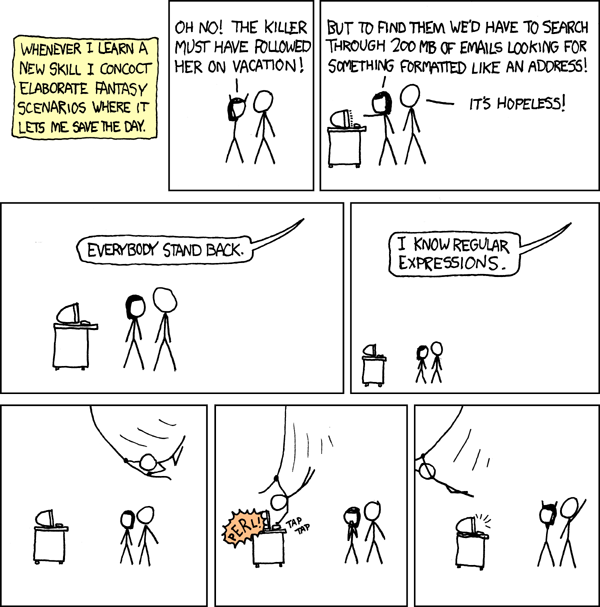
\includegraphics[width=220pt]{regular_expressions.png}
    \end{center}
  \end{figure}
  \begin{center}
    {\tiny Wait, forgot to escape a space.  Wheeeeee[taptaptap]eeeeee.}
  \end{center}
\end{frame}

\end{document}
